\documentclass[letterpaper,twocolumn,10pt]{article}
\usepackage{epsfig,xspace,url}
\usepackage{authblk}
\usepackage{graphicx}
\usepackage{booktabs}

\title{Course Project\\
Characterizing LoRa Reliability and Throughput Under Range and Obstruction Constraints}
\author{Rodrigo Cahuana}

\begin{document}

\maketitle

\subsection*{Introduction}
LoRa is attractive for wireless sensing because it can trade data rate for range, but that tradeoff is only useful if the link remains reliable in realistic obstructed environments. This project evaluates a point-to-point LoRa link at 915~MHz using controlled field tests that vary distance, obstruction, and spreading factor (SF). Our methodology keeps bandwidth, coding rate, transmit power, payload size, and packet generation rate fixed while measuring packet reception ratio (PRR), goodput, RSSI, SNR, burst loss, and timing jitter from logged receiver traces. The main result is that SF12 was the most reliable setting for the long obstructed links: it achieved 100\% PRR in both 1-mile trials and 0.86--0.95 PRR in the usable 2-mile trials, while SF7 delivered much higher goodput but became inconsistent and bursty as the path became harder. In short, the experiments show a clear throughput-versus-robustness tradeoff that matches the expected LoRa design space.

\subsection*{Related Work}
Prior LoRa and LPWAN literature explains why this tradeoff should appear. Centenaro et al.\ describe LoRa as a low-power wide-area technology that exchanges spectral efficiency for long-range connectivity in sub-GHz bands~[1]. Semtech's LoRa modulation note explains that increasing SF raises receiver sensitivity and range at the cost of airtime and data rate~[2]. Bor et al.\ show that airtime growth and shared-medium contention can also limit LoRa scalability, making parameter selection important even when links are technically decodable~[3]. The LoRaWAN specification formalizes the parameter set used in deployed systems~[4]. Our contribution is narrower and experimental: instead of proposing a new MAC or protocol, we built a small measurement framework and used it to characterize how SF7, SF10, and SF12 behave on the same obstructed paths using the same packet source and analysis pipeline.

\subsection*{Methodology}
The testbed uses one LoRa transmitter and one LoRa receiver implemented on Heltec LoRa development boards. The receiver stays attached to a laptop over USB serial, while the transmitter is powered from a battery pack so it can be moved to different locations. All experiments use the same base radio settings unless otherwise noted: 915~MHz carrier frequency, 125~kHz bandwidth, coding rate 4/5, transmit power 14~dBm, 20-byte payloads, and a packet period of 200~ms (5 packets/s).

The transmitter embeds a sequence number in every payload. The receiver logs each decoded packet together with RSSI, SNR, packet length, and timing metadata. Offline scripts summarize each CSV trace into PRR, estimated missed packets, average goodput, PHY bitrate, airtime, channel occupancy, burst-loss statistics, and inter-arrival jitter. This made it possible to compare not only whether a link worked, but also how gracefully it failed when the path degraded.

We used two completed experiment phases in the final report. First, bring-up tests at 2~m and 10~m line-of-sight verified that the hardware and logging chain worked correctly. Second, long-range obstructed tests at roughly 1 mile and 2 miles compared SF7, SF10, and SF12, including repeats to assess stability. Short accidental captures were retained in the repository for completeness, but the discussion below emphasizes the longer runs that lasted tens of seconds and therefore better represent sustained link behavior.

\subsection*{Implementation}
The firmware consists of a transmitter sketch and a receiver sketch, with separate builds for SF7, SF10, and SF12. The transmitter sends fixed-size packets containing a monotonically increasing sequence number. The receiver decodes each packet, estimates missing sequence numbers, and streams CSV-formatted records over serial. This design avoids putting analysis logic on the radio node and keeps the on-device software simple.

The host-side tooling automates the rest of the workflow. PowerShell scripts launch each experiment, save the raw CSV logs under the appropriate \texttt{data/} subdirectory, and run analysis scripts that generate summary tables and plots under \texttt{results/}. The submitted code artifact is the accompanying repository used for this report; the firmware is under \texttt{firmware/} and the logging and analysis scripts are under \texttt{scripts/}. Code available at: \url{https://github.com/rcahuana987/ecen526-lora-project}. No code is reproduced in this paper, consistent with the course instructions.

\subsection*{Experimentation}
The bring-up phase established a clean baseline. At both 2~m and 10~m line-of-sight using SF7, the link achieved PRR~=~1.00, mean RSSI near $-14.5$~dBm, mean SNR about 12.3--12.4~dB, and goodput near 100.7~B/s. That gave confidence that later losses came from the channel and geometry rather than from basic implementation errors.

Table~\ref{tab:longrange} summarizes the long-range results. At 1 mile with obstructions, SF12 was the clear reliability winner: both runs achieved PRR~=~1.00 with no observed burst losses, although the higher airtime reduced goodput to about 15.5~B/s. SF10 behaved as a middle point: one run reached 0.974 PRR, but the repeat fell to 0.553 and showed a 17-packet loss burst. SF7 delivered the highest goodput (roughly 51--87~B/s) but was much less stable, with PRR from 0.50 to 0.86 and one repeat containing a 104-packet burst loss. This is the practical tradeoff the project set out to measure.

At 2 miles, the pattern became stronger. SF12 remained usable over long captures, reaching PRR from 0.862 to 0.950 with goodput around 13.4--15.1~B/s even though the mean SNR was around $-15$ to $-17$~dB. SF10 became inconsistent; the longer run captured only 6 of 15 packets (PRR~=~0.40), while a separate very short capture decoded two packets but is not strong evidence of sustained performance. SF7 was effectively unusable at this distance in the available data, with only three packets captured in a short run. Figures~\ref{fig:prr} and~\ref{fig:tradeoff} visualize the same trend: higher SF improves long-range reliability, but it does so by sharply increasing airtime and reducing throughput.

\begin{table}[t]
\centering
\caption{Representative long-range results from the logged traces.}
\label{tab:longrange}
\begin{tabular}{llll}
\toprule
Path & SF & PRR & Goodput (B/s) \\
\midrule
1 mile obstacle & 7  & 0.50--0.86 & 50.7--86.7 \\
1 mile obstacle & 10 & 0.55--0.97 & 29.3--51.7 \\
1 mile obstacle & 12 & 1.00       & 15.5       \\
2 mile obstacle & 7  & link unstable & 75.0$^\dagger$ \\
2 mile obstacle & 10 & 0.40 in long run & 22.6 \\
2 mile obstacle & 12 & 0.86--0.95 & 13.4--15.1 \\
\bottomrule
\end{tabular}

\vspace{1mm}
\footnotesize{$^\dagger$ Based on a short capture, so the goodput value is less meaningful than the reliability trend.}
\end{table}

\begin{figure}[t]
\centering
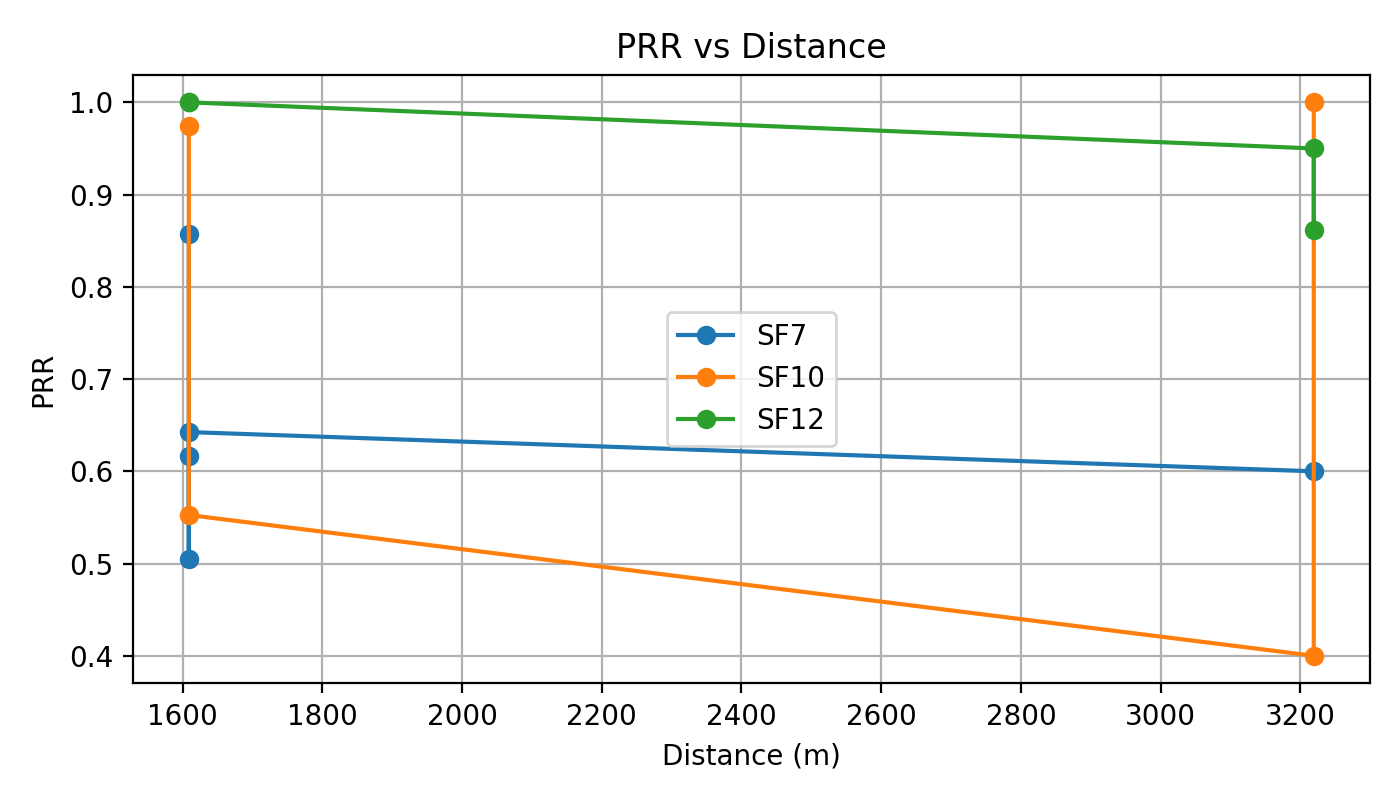
\includegraphics[width=\columnwidth]{../results/02_sf_tradeoff/prr_vs_distance.png}
\caption{PRR across distance for the measured spreading factors.}
\label{fig:prr}
\end{figure}

\begin{figure}[t]
\centering
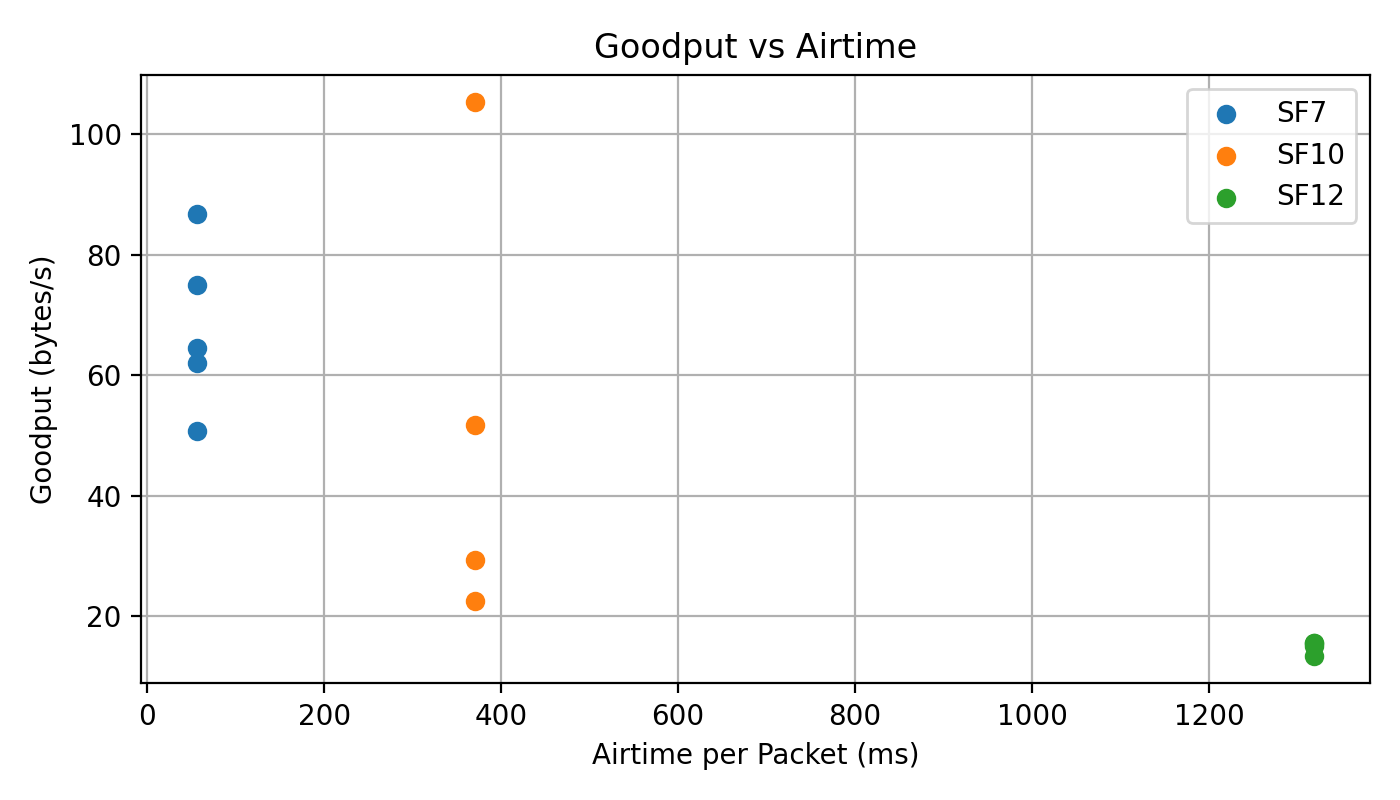
\includegraphics[width=\columnwidth]{../results/02_sf_tradeoff/goodput_vs_airtime.png}
\caption{The measured throughput-versus-airtime tradeoff.}
\label{fig:tradeoff}
\end{figure}

An additional observation is that reliability should not be judged by PRR alone. The SF7 and SF10 repeats sometimes had acceptable average PRR but still experienced large burst losses and timing irregularity, which would matter to a sensing or telemetry application expecting steady updates. The summary scripts therefore proved useful because they exposed failure modes that a simple packet count would hide.

\subsection*{Conclusion}
This project built a complete measurement pipeline for point-to-point LoRa testing and used it to compare three spreading factors on short and long obstructed paths. The main conclusion is that SF12 provided the most robust link on the measured 1-mile and 2-mile routes, while SF7 provided the highest throughput but suffered the most instability and burst loss. SF10 occupied the middle ground, but its repeatability was weaker than expected on the obstructed path. The experiments therefore support the usual LoRa intuition: aggressive settings are attractive when the channel is easy, but conservative settings are better once range and blockage dominate.

Future work could extend the study in three directions. First, the dataset should be expanded with more repeated runs at fixed locations so that outliers and accidental short captures can be filtered statistically instead of manually. Second, the dropped obstacle-only phase should be completed to isolate the effect of walls and corners separately from pure range. Third, adaptive-rate or adaptive-power logic could be added so the link automatically selects the best operating point rather than relying on manually reflashed firmware.

\subsection*{References}
\begin{enumerate}
\item M. Centenaro, L. Vangelista, A. Zanella, and M. Zorzi, ``Long-range communications in unlicensed bands: the rising stars in the IoT and smart city scenarios,'' \emph{IEEE Wireless Communications}, vol.~23, no.~5, pp.~60--67, 2016.
\item Semtech Corporation, ``AN1200.22 LoRa Modulation Basics,'' application note, Rev.~2, May 2015. Available: \url{https://www.semtech.com/uploads/documents/an1200.22.pdf}
\item M. Bor, U. Roedig, T. Voigt, and J. M. Alonso, ``Do LoRa low-power wide-area networks scale?,'' in \emph{Proceedings of the 19th ACM International Conference on Modeling, Analysis and Simulation of Wireless and Mobile Systems (MSWiM)}, 2016, pp.~59--67.
\item LoRa Alliance, ``LoRaWAN Specification,'' 2015. Available: \url{https://lora-alliance.org/resource_hub/lorawan-specification-v1-0/}
\item J. Gromes and M. Krizan, ``RadioLib: Universal wireless communication library for embedded devices.'' Available: \url{https://github.com/jgromes/RadioLib}
\end{enumerate}

\end{document}
